\documentclass[12pt]{scrbook}
\usepackage[charter]{mathdesign}
\usepackage{amsmath}
\usepackage{appendix}
\usepackage{amsthm}
\usepackage{pgfplots}


\newtheorem*{definition}{Definition}
\newtheorem{lemma}{Lemma}[section]
\newtheorem{proposition}{Proposition}[section]
\newtheorem{theorem}{Theorem}[section]
\newtheorem{corollary}{Corollary}[section]

\begin{document}

\title{Real and Complex Analysis}
\author{Dr Ahmed Riza}
\date{}
\maketitle

\tableofcontents

\chapter{Real Numbers}

\section{Bounded Sets of Numbers}

\begin{definition}
The Greatest and Least members of a Set: If S is a set consisting of finitely many different real numbers, plainly there is one member of the set which is greater than all the others and one member which is less than all the others.  Convenient abbreviations for these greatest and least numbers are MAX and MIN.
\end{definition}

If now S is a set with infinitely many members, there may or may not be a member of S which is greater than all the others (or one which is less than all the others).

\begin{definition}
Let S be a set of real numbers.  If there is a number K such that, for every member $x$ of $S$, $ x \leq K$, we say that $S$ is bounded above. K is called an {\em upper bound} of S.  Similarly, if there is a K such that $x \ge K$ for every $x \in S$, then S is said to be bounded below, and K is a {\em lower bound} of S.

If S is bounded both above and below, we say simply that it is {\em bounded}. A set which is not bounded is called {\em unbounded}.
\end{definition}

\begin{theorem} % 1.8 Burkhill
\label{theorem-1.8}
If S is a (non-empt) set of numbers which is bounded above, then of all the upper bounds, there is a least one.
\end{theorem}

\begin{proof}
Divide the real numbers x into two classes L, R by these rules:

Put x in L if there is a member s of S such that $s > x$.

Put x in R if, whatever member s of S is taken, $s \leq x$.

Then every x goes either into L or into R.  Moreover, neither L nor R is empty.  For, if s is some member of S, then (say) $ x = s - 1 $ is in L.

And, since S is bounded above, any upper bound K, for which $s \leq K$ for all s, is in R. 

Any l of L is less than any r of R.  For there is some s which is greater than l, and this s is less than or equal to r.

By Dedekind's axiom, there is a dividing number $\xi$ such that, for every positive $\epsilon$, $\xi - \epsilon$ is in L and $\xi + \epsilon$ is in R.  In the Dedekind axiom, $\xi$ itself may belong either to L or to R.  We shall prove that, in the present application, $\xi$ belongs to R.

Suppose, if possible, that $\xi$ belongs to L.  Then there is a member s of S which $s > \xi$.

The number $\eta = \frac{1}{2}(s + \xi)$ satisfies $ s > \eta > \xi$: $\eta$ is in R since it is greater than the dividing number $\xi$. So $s \leq \eta$ by the rule for R.  This contradicts our earlier inequality $s > \eta$. So $\xi$ belongs to R.  We have proved that $\xi$ satisfies
\begin{enumerate}
	\item $s \leq \xi$ for every s in S
	\item $\xi - \epsilon$ being any number less than $\xi$, tree is an s for which $s > \xi - \epsilon$.
\end{enumerate}
The property (1) shows that $\xi$ is an upper bound of S, and (2) that it is the least upper bound.  
\end{proof}

\begin{definition}
\label{def-supremum}
If, given a set of numbers S, there is a number K such that
\begin{enumerate}
	\item $s \leq K$ for every s in S
	\item for every positive $\epsilon$, there is an s in S for which $s > K - \epsilon$, then we write $K = \sup S$.
\end{enumerate}
\end{definition}

Theorem~\ref{theorem-1.8} proved the existence of K when the set S is bounded above. 

By reversing inequality signs, we set up an analogous theory of lower bounds and the greatest of the lower bounds (the {\em infinimum}, abbreviated $\inf$). 

\begin{definition}
\label{def-infinimum}
If, given a set of numbers S, there is a number k such that 
\begin{enumerate}
	\item $s \ge k$ for every s in S
	\item for every positive $\epsilon$, there is an s in S for which $s < k + \epsilon$, then we write $k = \inf S$.
\end{enumerate}
\end{definition}

A set which is bounded below can be proved to have an infinimum.

\subsection{Examples}

\begin{enumerate}
	\item Let S be the rational numbers x for which $0 \leq x \leq \frac{1}{2}$. Then $\frac{1}{2}$ is the least upper bound.  It is also the greatest member of S.
	
	\item Let S be the rational numbers x for which $x^2 < 2$.  The number $\sqrt{2}$ is the least upper bound.
	
	\item Let S denote the set of all rational numbers r satisfying $r \leq 3$.  Show that 3 is the $\sup(S)$.  In this case, $3 \in S$, so S includes its least upper bound. 
	
	From the given inequality $r \leq 3$, so that part (1) of Definition~\ref{def-supremum} is satisfied.  Now whatever the value of $\beta >0$, $3 > l - \beta$ and $3 \in S$ so that part (2) of the definition is satisfied.  Hence 3 is the l.u.b for S.
	
	\item Let S denote the set of rational numbers satisfying $x < 6$.  Then S has no largest member.
	
	The number 6 is not the largest member of S because it does not belong to S, and indeed no number greater than 6 belongs to S. On the other hand if $l$ is a member of S which is less than 6 then the number $(l + 6)/2$ is a rational number which is greater than $l$, and less than 6, so that it is a member of S.  So $l$ could not be the largest member of S. This demonstrates that S has no largest member.
	
	\item Let S denote the set of all rational numbers whose squares are less than 2.  Then S is a bounded set but it has no largest member.
	
	If $x \ge 2$ then $x^2 \ge 4 > 2$, and so $x \notin S$.  Hence, the number 2 is an upper bound for S.  It is clearly not the least upper bound, as a similar argument demonstrates that 3/2, for example, is also an upper bound for S.  Similarly, -2 is a lower bound for S, so that S is a bounded set.  Suppose that $l$ were the largest member of S.  We cannot have $l^2 = 2$, for there is no such rational number, as we have shown.  We cannot have $l^2 > 2$ for then $l \notin S$.  We shall show that $l^2 < 2$ is also impossible.
	
	If $l^2 < 2$ we shall show that we can find a larger number $l + \alpha, (\alpha > 0)$ whose square is also less than 2, as follows:
	
	\begin{eqnarray*}
	(l + \alpha)^2 	&=& l^2 + 2 l \alpha  + \alpha^2 \\
				&<& l^2 + 4 \alpha + \alpha^2 \;\;\; \text{since} \; l < 2 \\
				&<&  l^2 + 5 \alpha \;\;\; \text{provided} \; \alpha < l \\
				&<&  2 \;\;\;  \text{provided} \; \alpha < (2 - l^2)/5
	\end{eqnarray*}
	
	
	\item Let A and B be sets of numbers which are bounded above, with l.u.b $a$ and $b$ respectively.  Let C denote the set of all numbers of the form $x + y$, where $x \in A$ and $y \in B$.  Show that the l.u.b of C is $a + b$.
	
	For all $x \in A$ and $y \in B$, $x \leq a$ and $y \leq b$, using part (1) of the definition of l.u.b.  Hence, $x + y \leq a + b$, and so $a + b$ is an upper bound for C.  We now apply part (2) of the definition of l.u.b to A and to B, with $\beta$ replaced by $\beta/2$.  So for any positive number $\beta$, there are numbers $x \in A$ and $y \in B$ satisfying $x > a - \beta/2$ and $y > b - \beta/2$.  Thus, $ x + y > a + b - \beta $ and so we have shown that there is a number in C exceeding $ a + b - \beta $.  So part (2) of the definition is satisfied, showing that $a + b$ is the l.u.b for C.
	
\end{enumerate}

\section{Axiom of Completeness for the Real Number System}

\begin{definition}
	This states that every non-empty set of real numbers which is bounded above must have a least upper bound in the set of real numbers.  See Theorem~\ref{theorem-1.8} for proof.
\end{definition}

\begin{proposition}
\label{prop-sqrt-two}
There is a real number satisfying the equation $x^2 = 2$.
\end{proposition}

\begin{proof}
We consider the set of all rational numbers $r$ satisfying $r^2 < 2$.  We know that this set is bounded above, and the axiom of completeness says that S must have a least upper bound $l$.  We shall show that $l^2 = 2$ by demonstrating that $l^2 < 2$ and $l^2 > 2$ are both impossible.

In a previous example, we showed that if $l^2 < 2$, then we can find a larger number $l + \alpha$ whose square is also less than 2, implying that $l$ could not be an upper bound for S.  Now suppose that $l^2 > 2$.  We shall show that there is a number of the form $l - \beta$ where $\beta > 0$ whose square is also greater than 2.  This will mean that  $l - \beta$ is also an upper bound, so that $l$ could not be the {\em least} upper bound. Now

	\begin{eqnarray*}
	(l  - \beta)^2 	&=& l^2 - 2 l \beta - \beta^2 \\
				&>& l^2 - 4 \beta \;\;\; (\text{since} \; \beta^2 > 0 \; \text{and} \; l < 2) \\
				&>&  2 \;\;\;  \text{provided} \; \beta < (l^2 - 2)/4
	\end{eqnarray*}
	
So we have shown that there is a real number whose square is 2, finally legitimising the use of the symbol $\sqrt{2}$ for the number $l$ defined above.
\end{proof}

\begin{proposition}
There is a unique positive real number satisfying the equation $x^2 = 2$.
\end{proposition}

\begin{proof}
Existence was established in Proposition~\ref{prop-sqrt-two}.  Here we are demonstrating uniqueness.  The proof uses the method of contradiction.  Suppose that $x_1$ and $x_2$ are both positive numbers satisfying $x^2 = 2$.  Then $x_1^2 = x_2^2$, and so $x_1^2 - x_2^2 = 0$.  Factorizing this gives $(x_1 + x_2)(x_1 - x_2) = 0$.  We must therefore have $(x_1 + x_2) = 0$ or $(x_1 - x_2) = 0$. Since $x_1$ and $x_2$ are both positive we cannot have $(x_1 + x_2) = 0$.  Hence $(x_1 - x_2) = 0$ and so $x_1 = x_2$, proving uniqueness.
\end{proof}

\begin{proposition}
Given any two positive real numbers $a$ and $b$, there is a positive integer $n$ satisfying $na \geq b$.  This is known as the {\bf Archimedean Property}.
\end{proposition}

\begin{proof}
As on so many occasions, the proof employs the method of contradiction.  So we suppose that the result is false, i.e. that there are two real numbers $a$ and $b$ such that for every positive integer $n, na < b$. This means that the set S of numbers of the form $na$ is bounded above by $b$.  S therefore has a least upper bound $l$.  Now, $l - a < l$ and so there is a number of the set S between $l - a$ and $l$, i.e. there is a positive integer $n_0$ satisfying $l - a < n_0 a < l$.  Adding $a$ to each side of the left-hand inequality gives $l < (n_0 + 1)a$, giving a number of S greater than $l$.  This is a contradiction.
\end{proof}

\begin{proposition}
Between any two real numbers there are both rational and irrational numbers.
\end{proposition}

\begin{proof}

\end{proof}

%%%%%%%%%%%%%%%%%%%%%%%%%%%%%%%%%%%%%%%%%%%%%%%%%%%%%%%%%%%%%%%%%%%%%%%%

\chapter{Absolute Value, Complex Numbers and Inequalities}

\section{Absolute Value}

\[ |x| = \text{max}(x, -x) \]
Equivalently:
\[ |x| = \sqrt{x^2} \]
$|x - y|$ is the distance between $x$ and $y$. Example, if $x = -5$ and $y = 4$, then 
\[ |x-y| = |-5-4| = |-9| = 9 \]

\subsection{Example}
Fix $x_0 \in \mathbb{R} \;\;\; \epsilon > 0$.
\[ \{ x \in \mathbb{R} : |x - x_0| < \epsilon \} \]

Algebraically:
\[ |x - x_0| < \epsilon \Leftrightarrow \text{max}(x - x_0, x_0 - x) < \epsilon \]

There are two cases:

\[ x - x_0 > 0 \Rightarrow \text{max}(x - x_0, x_0 - x) = x - x_0 < \epsilon \]

\[ x < x_0 \Rightarrow \text{max}(x - x_0, x_0 - x) = x_0 - x < \epsilon \]

\[ \Rightarrow x_0 - \epsilon < x < x_0 + \epsilon \]

\section{Complex Numbers}

Let $z = x + iy \;\;\; x, y \in \mathbb{R} $. $ |z| $ is the distance of $z$ to the origin and equals
\[ \sqrt{x^2 + y^2} \]

$|z - w|$ is the distance of $z$ to $w$.

\section{Triangle Inequality}

\begin{theorem}
\[ |z - w| \le |z| + |w| \]
Equivalent to 
\[ |z + w| \le |z| + |w| \]
\end{theorem}

\begin{proof}
\begin{eqnarray*}
| z + w |^2 &=& (z + w)^2 = z^2 + 2zw + w^2 \\
                  &\le& |z|^2 + 2|z||w| + |w|^2 = (|z| + |w|)^2
\end{eqnarray*}
\[ \Rightarrow |z + w| \le |z| + |w| \]
\end{proof}

\section{Reverse Triangle Inequality}

\begin{theorem}
\[ |z - w| \ge \left| |z| - |w| \right| \]
\end{theorem}

\begin{proof}

\begin{eqnarray*}
|z - w| + |w| &\ge& |z - w + w | = |z| \\
|w - z| + |z|  &\ge&  |w - z + z | = |w| 
\end{eqnarray*}
This can be re-written as
\begin{eqnarray*}
|z - w| &\ge& |z - w + w | = |z| - |w| \\
|w - z|   &\ge&  |w - z + z | = |w| - |z| 
\end{eqnarray*}
Now, $|z - w| = |w - z|$ and if $t \ge a$ and $t \ge -a$, then $t \ge |a|$.  Using this, we can conclude

\[ |z - w| \ge \left| |z| - |w| \right| \]

\end{proof}

\section{Bernoulli Inequality}

The following inequality is very important in analysis.

\[ (1 + x)^n \ge 1 + nx \;\;\; \text{for} \;\;\; x > -1 \;\;\; \text{and} \;\;\; n \in \mathbb{N} \]

\begin{proof}
We use induction on $n$.  If $n = 0$
\[ (1 + x)^0 \ge 1 + 0(x) \Rightarrow 1 \ge 1 \]
is trivially true.  Assume it is true for $n = k$ for some $k$, i.e.
\[ (1 + x)^k \ge 1 + kx \]

\[ (1+x)(1 + x)^k \ge (1+x)(1 + kx) \]
This is true, since $x > -1$ and $(1 + x) > 0$.

\begin{eqnarray*}
\Rightarrow (1+x)^{k+1}  &\ge&  1 + x + kx + kx^2 \\
                                       &\ge& 1 + (k+1)x + kx^2 \\
                                       &\ge& 1 + (k+1)x
\end{eqnarray*}
since $kx^2 > 0$.
Therefore, by induction, the statement is true for all $n \in \mathbb{N}$.

\end{proof}

%%%%%%%%%%%%%%%%%%%%%%%%%%%%%%%%%%%%%%%%%%%%%%%%%%%%%%%%%%%%%%%%%%%%%%%%

\chapter{Sequences}

A sequence is a countable set of real or complex numbers written down in some order.

\[ \frac{1}{2}, \frac{1}{4}, \ldots , \frac{1}{2^n}  \]

\[ 1, -1, 1, -1, \ldots , (-1)^{n-1} \]

\[ 3, 9, 27, \ldots , 3^n \]

\begin{definition}
A real or complex sequence is a mapping
\[ S : \mathbb{N} \rightarrow \mathbb{R} \;\;\; \text{or} \;\;\; \mathbb{C} \]
\end{definition}

$S_n$ is the $n^{th}$ term of the sequence, also used to denote the sequence itself. For example, $S_n = \frac{1}{n}$ designates the sequence
\[ 1, \frac{1}{2}, \frac{1}{3},  \frac{1}{4}, \ldots , \frac{1}{n} \]

Lets take $S_n = \frac{1}{n^2}$.  As $n$ increases the $n^{th}$ term tends to 0.  However, $S_n = (-1)^{n-1}$ does not tend to a single number as $n$ increases. $S_n  = 3^n$ runs away as $n$ increases and goes to infinity.

\section{Null Sequences}

\begin{definition}
A sequence is called a null sequence if for any $\epsilon > 0$, there exists an index $N \in \mathbb{N}$ (depending on $\epsilon$), such that for all $n > N$, we have $|S_n| < \epsilon$.
\end{definition}

\subsection{Example}
$S_n = \frac{1}{2^n}$ is a null sequence.  Let $\epsilon > 0$ be arbitrary, and take $N$ equal to some natural number such that $2^N > \frac{1}{\epsilon} \Leftrightarrow N > \log(1/\epsilon)$.

Then if $n \ge N \Rightarrow 2^n > 2^N > 1/\epsilon \Rightarrow \frac{1}{2^n} < \epsilon$.  But 
$\frac{1}{2^n} = |\frac{1}{2^n}| = S_n$.  So, for all $n > N$, $|S_n| < \epsilon$.  For example, take $\epsilon = \frac{1}{2^1000}$.
We can choose $N = 1001$ or $N = 2000$ etc.

Same argument shows that
\[ S_n = \frac{(-1)^n}{2^n} \]
is a null sequence, since
\[ S_n = \left| \frac{(-1)^n}{2^n} \right| = \frac{1}{2^n} \]

\subsection{Example}

\[
S_n = 
  \begin{cases}
    0 & \text{if n is odd} \\
    1 & \text{if n is even}
  \end{cases}
\]
is not a null sequence.
\begin{proof}
Suppose it were a null sequence.  Then applythe definition, with $\epsilon = \frac{1}{2}$.  Then there should exist an $N$ such that if $n > N$, then $|S_n| < \frac{1}{2}$.  But this gives a contradiction, if we take an $n > N$, which is even (e.g. $n = 2N$).  
Then $|S_n| = 1 > \frac{1}{2}$.  Hence it is not a null sequence.
\end{proof}

\section{Sequences Having a Limit (Converging Sequences)}

\begin{definition}
A sequence $S_n$ tends to a limit $L$, if for all $\epsilon > 0$, there eixts an $N$ (depending on $\epsilon$), such that for 
all $n > N$, 
\[ \left| S_n - L \right| < \epsilon \]
\end{definition}

Remarks:
\begin{itemize}
\item $S_n$ tneds to $L$ if and only if $S_n - L$ is a null sequence.
\item $S_n$ is a null sequence if and only if $S_n$ tends to 0.
\end{itemize}

\subsection{Example}
\[ S_n = \frac{n+1}{n} = 1 + \frac{1}{n} \]

\[ S_n - 1 = \frac{1}{n} \]
is a null sequence, so $S_n \rightarrow 1$.

Or, using the definition:

\[ \left|S_n - 1 \right| = \left| \frac{n+1}{n} - 1 \right| = \left| \frac{n+1-n}{n} \right| = \frac{1}{n} \]
We want
\[ \frac{1}{n} < \epsilon \Leftrightarrow n > \frac{1}{\epsilon} \]
So, for any $\epsilon > 0$, let $N$ be any natural number $> \frac{1}{\epsilon}$.  Then if 
\[ n > N \Rightarrow \frac{1}{n} < \frac{1}{N} < \epsilon \]
So, 
\[ n > N \Rightarrow \left|  S_n - 1 \right| < \epsilon \]
Since $\epsilon > 0$ is arbitrary, this shows that
\[ \lim_{n \to \infty} \frac{n+1}{n} = 1 \]


\section{Properties of Limits}

\begin{lemma}
\label{lemma-lim-1}
If $x_n$ and $y_n$ are null sequences, then so is $x_n + y_n$.
\end{lemma}

\begin{proof}
Let $\epsilon > 0$ be arbitrary.  Since $x_n \rightarrow 0$, there exits an $N_1$ such that if $n > N_1$, then 
$|x_n| < \frac{\epsilon}{2}$.

Since $y_n \rightarrow 0$, there exists $N_2$ such that if $n > N_2$, then $|y_n| < \frac{\epsilon}{2}$. If 
$n > \text{max}\{N_1, N_2\}$, then $\left| x_n + y_n \right| \le |x_n| + |y_n| < \frac{\epsilon}{2} + \frac{\epsilon}{2} = \epsilon$.

So, we have shown that there exists an $N$ such that for all $n > N$, 
\[ \left| x_n + y_n \right| < \epsilon \Rightarrow x_n + y_n \rightarrow 0 \]
\end{proof}

%%%%%%

\begin{lemma}
\label{lemma-lim-2}
If $x_n$ is a null sequence ($x_n \rightarrow 0$) and $y_n$ is a bounded sequence, then $x_n y_n$ is again a null sequence.
\end{lemma}

\begin{proof}
$y_n$ is bounded, so there exists a number $k$ such that $|y_n| \le k$ for all n.

\[ \left| x_n y_n \right| \le k|x_n| < \epsilon \Leftrightarrow |x_n| < \frac{\epsilon}{k} \]

Now, $x_n \rightarrow 0$, so applying the definition with $\epsilon/k$ instead of $\epsilon$, there exists $N$ such that
\[ n > N \Rightarrow |x_n| < \frac{\epsilon}{k} \]

But then, if $n > N$, then
\[ \left| x_n y_n \right| \le k|x_n| < k \frac{\epsilon}{k} = \epsilon \]

So, for any $\epsilon > 0$, we can find an $N$ such that
\[ \left| x_n y_n \right| < \epsilon \Rightarrow x_n y_n \rightarrow 0 \]

\end{proof}

%%%%%%

\begin{lemma}
\label{lemma-lim-3}
Suppose a sequence $t_n$ has a limit, then $t_n$ is a bounded sequence, i.e., there exists a $k > 0$ such that 
\[ |t_n| < k \;\;\; \forall n \]
\end{lemma}

\begin{proof}
Suppose $t_n \rightarrow t$. Apply the definition with $\epsilon = 1$.

\[ \exists \; N: n > N \Rightarrow \left| t_n - t \right| < 1 \]
\[ |t_n| = \left| t_n - t + t \right| \le \left| t_n - t \right| + |t| < 1 + |t| \;\;\; \forall n > N \]

If $n \le N$, then 
\[ | t_n | \le \max\left( |t_1|, |t_2|, \ldots , |t_N| \right) \]

So
\[ |t_n| \le \max\left( |t_1|, |t_2|, \ldots , |t_N|, 1 + |t| \right) = k \;\;\; \forall n \]

\end{proof}

%%%%%%

\begin{theorem}
Suppose $s_n \rightarrow s$ and $t_n \rightarrow t$. Then
\begin{enumerate}
\item $ s_n + t_n \rightarrow s + t $
\item $ s_n t_n \rightarrow s t $
\item $ \frac{s_n}{t_n} \rightarrow \frac{s}{t} $ provided $t_n \ne 0$ and $t \ne 0$.
\end{enumerate}
\end{theorem}

\begin{proof}
\begin{enumerate}
\item
\[ s_n - s \rightarrow 0 \;\;\; t_n - t \rightarrow 0 \]
Apply Lemma~\ref{lemma-lim-1} to $x_n = s_n - s$ and $y_n = t_n - t$.

\[ (s_n - s) + (t_n - t) = (s_n + t_n) - (s + t) \rightarrow 0 \]
Hence $s_n + t_n \rightarrow s + t$.

\item 
\[ s_n \rightarrow s \;\;\; t_n \rightarrow t \]
We want to show that $s_n t_n \rightarrow s t$ or equivalently $s_n t_n - s t \rightarrow 0$.

\[ s_n t_n - s t = (s_n - s)t_n + s(t_n - t) \]

$t_n \rightarrow t$, so $t_n$ is a bounded sequence (Lemma~\ref{lemma-lim-3}).  $s_n \rightarrow s$, so $s_n - s$ is a null sequence.  From Lemma~\ref{lemma-lim-2}, $(s_n - s)t_n$ is a null sequence, i.e., $(s_n - s)t_n \rightarrow 0$.

$t_n \rightarrow t$, so $t_n - t$ is a null sequence. The sequence which is constant and equal to $s$ is bounded.  By Lemma~\ref{lemma-lim-2}, $s(t_n - t) \rightarrow 0$.

Since the sum of a null sequence is a null sequence, we get 
\[ (s_n - s)t_n + s(t_n - t) \rightarrow 0 \]
Hence
\[ s_n t_n \rightarrow s t \]

\item  We will prove this part in several stages.

\begin{enumerate}
\item Explain why 
\[\left| \frac{1}{b_n} - \frac{1}{b} \right| = \frac{1}{|b_n b|} \left| b_n - b \right| \]
We can write the left hand side as:
\[ \left| \frac{1}{b_n} - \frac{1}{b} \right| = \left| \frac{b - b_n}{b_n b} \right|  = \frac{1}{|b_n b|} \left| b_n - b \right| \]
since $|b - b_n| = |b_n - b|$.

\item Show in two steps that the sequence, $\left\{ \frac{1}{|b_n b|} \right\}$ is bounded.
\begin{enumerate}
\item Show that the set $\{ b_n \}$ is bounded away from zero, i.e., there is some $\delta > 0$ such that 
$|b_n| \ge \delta$ for all $n$.

We know that
\[ b_n \rightarrow b \Rightarrow \exists N: |b_n - b| < \epsilon \;\;\; \forall n > N \]
Let $\epsilon = \frac{|b|}{2} > 0$.  It follows that
\[ |b_n - b| < \frac{|b|}{2} \]
Using the reverse triangle inequality
\begin{eqnarray*}
|b_n - b| &\ge& \left| |b_n| - |b| \right| \\
              &\ge& \left| |b| - |b_n| \right| 
\end{eqnarray*}
Using this, we have
\[ |b| - |b_n| < \frac{|b|}{2} \Rightarrow b_n > \frac{|b|}{2} \;\;\; \forall n > N \] 

The remaining set $S = \{ |b_1|,  |b_2|,  \ldots, |b_N| \}$ is a finite set of positive numbers, and so has a positive minimum. 
We can choose our $\delta = \min(S)$ and conclude that
\[ |b_n| \ge \delta \;\;\; \forall n, \delta > 0 \]

\item Show that 
\[ \frac{1}{|b_n b|} < \frac{2}{(\delta |b|)} \;\;\; \forall n \]

\[ |b_n| \ge \delta \Rightarrow |b_n b| \ge \delta |b| > \frac{\delta |b|}{2} \]
since $|b| > |b|/2$.

\[ \Rightarrow \frac{1}{|b_n b|} < \frac{2}{(\delta |b|)} \;\;\; \forall n \]

\end{enumerate}

\item We have shown in part (b) above that $\frac{1}{|b_n b|}$ is bounded.  Now prove that 
\[ \frac{1}{b_n}\rightarrow \frac{1}{b} \]

From part (a), we have
\[\left| \frac{1}{b_n} - \frac{1}{b} \right| = \frac{1}{|b_n b|} \left| b_n - b \right| \]

Since $\frac{1}{b_n b}$ is bounded above, say by $M$, that is, $\frac{1}{b_n b} < M$

\[\Rightarrow \left| \frac{1}{b_n} -\frac{1}{b} \right| < M | b_n - b | \]
Since $b_n \rightarrow b$, $b_n - b$ is a null sequence.  By the product rule, $M|b_n - b|$ is also a null sequence and hence,
\[ \Rightarrow \left| \frac{1}{b_n} - \frac{1}{b} \right| \rightarrow 0 \Rightarrow  \frac{1}{b_n}\rightarrow \frac{1}{b} \]

\end{enumerate}

Finally, we can use the product rule again to show that $\frac{s_n}{t_n} \rightarrow \frac{s}{t} $.  By part (c) we have shown that 
$\frac{1}{t_n} \rightarrow \frac{1}{t}$.  Now,
\[ \frac{s_n}{t_n}  = s_n \left( \frac{1}{t_n} \right) \rightarrow \frac{s}{t} \] 

\end{enumerate}
\end{proof}

\subsection{Example of an application of this theorem}

\[ S_n = \frac{n^2 + 4n - 3}{2n^2 + 3n + 5} = \frac{1 + 4/n + 3/n^2}{2 + 3/n + 5/n^2} \]

Now, $4/n \rightarrow 0$, $3/n^2 \rightarrow 0$, $3/n \rightarrow 0$, $5/n^2 \rightarrow 0$.  
Therefore $S_n \rightarrow \frac{1}{2}$.

\section{Divergence to Infinity}

\begin{definition}
$S_n \rightarrow \infty$ if, for any given real number $A > 0$, there exists an $N$ (depending on $A$) such that 
if $n > N$, then $S_n > A$.
\end{definition}

\begin{definition}
$S_n \rightarrow -\infty$ if, for any given real number $A > 0$, there exists an $N$ (depending on $A$) such that 
if $n > N$, then $S_n < -A$.
\end{definition}

\subsection{Example}
Take 
\[ S_n = n^2 \]
This sequence does not have a limit.  The general term $n^2$ becomes bigger than any given number if $n$ grows.
We say that 
\[ \lim_{n \to \infty} n^2 = \infty \;\;\; \text{or} \;\;\; n^2 \rightarrow \infty \]

\[ S_n = n^2 > A \Leftrightarrow n > \sqrt{A} \]
So, we can take for $N$ any natural number $> \sqrt{A}$.

\subsection{Remark}
\[ s_n + t_n \rightarrow s + t \]
remains valid, if $s_n \rightarrow \infty$, provided $t_n$ has a finite limit or $t_n \rightarrow \infty$, i.e.

\[ s_n \rightarrow \infty, \;\;\; t_n \rightarrow t \in \mathbb{R} \;\;\; \text{or} \;\;\; t_n \rightarrow \infty
\Rightarrow s_n + t_n \rightarrow \infty \]
However, this is not true if $t_n \rightarrow -\infty$, because $\infty + (-\infty)$ is not defined.

\section{Example}
\[ s_n = n, \;\;\; t_n = -n + a, \;\;\; a \in \mathbb{R} \]

$s_n \rightarrow \infty$ and $t_n \rightarrow -\infty$, whatever the value of $a$.  But note that $s_n + t_n = a$!

\section{Monotone Sequences}

\begin{definition}
$s_n$ is an increasing (decreasing) sequence if $s_{n+1} \ge s_n$ ($s_{n+1} \le s_n$).
\end{definition}

\begin{theorem}
\label{monotone}
Monotone and bounded sequeces have a limit.

Suppose that $s_n$ is an increasing sequence which is bounded from above, i.e. there exists a $K \in \mathbb{R}$
such that $s_n \le K$ for all $n$.  Then $s_n$ tends to a limit.

Similarly, if $s_n$ is a decreasing sequence which is bounded from below, i.e. $s_n \ge L$ for all $n$, for some
$L \in \mathbb{R}$, then $s_n$ also tends to a limit.
\end{theorem}

\begin{proof}
\begin{enumerate}
\item Increasing Case:

The set $s_n$ is bounded from above.  Put $s = \sup\{s_n\}$.  We claim that $s_n \rightarrow s$.

Let $\epsilon > 0$.  On the one hand, $s$ is an upper bound, so
\begin{equation}
\label{mono-1}
s_n \le s \;\;\; \forall n
\end{equation}
On the other hand, $s$ is the smallest upper bound, i.e. the least upper bound.  Hence $s - \epsilon$ is no longer
an upper bound.  Therefore, there exists at least one $N$ such that 
\[ s_N > s - \epsilon \]
but the sequence is increasing, so
\[ n > N \Rightarrow s_n > S_N > s - \epsilon \]
So, we have shown that 
\begin{equation}
\label{mono-2}
s_n > s - \epsilon \;\;\; \forall n > N
\end{equation}

By using Equations~\ref{mono-1} and \ref{mono-2}:
\begin{eqnarray*}
s - \epsilon &<& s_n \le s  \\
\epsilon - s &>& -s_n \ge -s  \\
\epsilon &>& s - s_n \ge 0 \Rightarrow 0 \le s - s_n < \epsilon \\
|s - s_n| &<& \epsilon \;\;\; \forall n > N
\end{eqnarray*}
Hence, 
\[ s_n \rightarrow s \]

\item Decreasing Case

If $s_n$ is decreasing and bounded from below, 
\[ s_n \ge A \;\;\; \forall n \]
then $-s_n$ is increasing and bounded from above.  
\[ -s_n \le -A \;\;\; \forall n \;\;\; \Rightarrow -s_n \rightarrow -s \Rightarrow s_n \rightarrow s \]

\end{enumerate}
\end{proof}

\subsection{Application: Sequenes Defined by a Recurrence Relation}

\[ f : \mathbb{R} \longrightarrow \mathbb{R} \]

\[ x_{n+1} = f(x_n) \]
$x_1$ is given (this is a one term recurrence relation).  
\begin{enumerate}
\item If $f$ is increasing, then the sequence $x_n$ is increasing
\item Next, if we can show that $x_n$ is bounded, then $\lim_{n \to \infty} x_n$ exists.
\end{enumerate}

How do we find $x = \lim_{n \to \infty} f(x_n)$?  Let $n \rightarrow \infty$ in $x_{n+1} = f(x_n)$.   Note that in order for this technique 
to apply, we need something like the following to apply:

\[\lim_{n \to \infty} f(x_n) = f(\lim_{n \to \infty} x_n) \]
This works in general if $f$ is continuous. Now:

\[ x_{n+1} \rightarrow x \]
\[ f(x_n) \rightarrow f(x) \]

\subsection{Example}
Suppose that $x_1 = 1$, and for $n \ge 1$, 
\[ x_{n+1} = \sqrt{1 + x_n} \]
Thus, $x_n$ begins with: $1, \sqrt{2}, \sqrt{1 + \sqrt{2}}, \sqrt{1 + \sqrt{1 + \sqrt{2}}}$, etc.  It is certainly not immediately clear
what the limit will be if it exists!  However, the first few terms do suggest that $x_n$ is increasing.  We prove this in general
using induction:  
\[ x_1 = 1 < \sqrt{2} = x_2 \]
Now, if $x_{n-1} < x_n$, then 
\[ x_n = \sqrt{1 + x_{n-1}} < \sqrt{1 + x_n} = x_{n+1} \]
Hence, $x_n$ is increasing, by induction.  Also, $x_1 < 2$, and if $x_n < 2$ then 
\[ x_{n+1} = \sqrt{1 + x_n} < \sqrt{1 + 2} = \sqrt{3} < 2 \]
So $x_n$ is bounded above by 2.

Thus, we have shown that $x_n$ is increasing and bounded above, hence $x = \lim_{n \to \infty} x_n$ exists in $\mathbb{R}$.
To find its value we first need to find 
\[ \lim_{n \to \infty} \sqrt{1 + x_n} \]
In fact, this limit is simply $\sqrt{1 + x}$.  To prove this, write

\[ \left| \sqrt{1 + x_n} - \sqrt{1 + x} \right|= \frac{\left| 1 + x_n - (1+x) \right|}{\sqrt{1+x_n} + \sqrt{1 + x}} < |x_n - x| \]
since $x_n$ and $x$ are positive, so the denominator is greater than 1.  But 
\[ x_n \rightarrow x \Rightarrow |x_n - x| < \epsilon, \;\;\; \epsilon > 0 \]
\[ \Rightarrow \left| \sqrt{1 + x_n} - \sqrt{1 + x} \right| < \epsilon \]
Hence 
$\sqrt{1 + x_n}  \rightarrow \sqrt{1 + x}$ as claimed.

Now, we have $x = \lim_{n \to \infty} x_n = \lim_{n \to \infty} x_{n+1} = \sqrt{1 + x}$. 
\[ x^2 - x - 1 = 0 \]
\[ \Rightarrow x = \frac{1 + \sqrt{5}}{2} \]
since $x > 0$.  This number is known as the golden section, which is also the limit of ratios of successive Fibonacci numbers.

\subsection{Example}
Consider the sequence given by 
\[ x_0 = a + 1, \;\;\; x_{n+1} = x_n \left( 1 + \frac{a - x_n^k}{k x_n^k} \right) \]
for a fixed $a > 0$ and fixed $k \in \mathbb{N}$. 

Let's try $a = 1$, $k = 1$.  
\[ \Rightarrow x_0 = 2 \Rightarrow x_1 = 2 \left( 1 + \frac{1-2}{2} \right) = 1 \]
So, we claim that $x_{n+1} < x_n$, $x_n > 0$ and $x_n^k > a$ (in order for the sequence to decrease).  Lets prove all three claims
by using induction. If $n = 0$:

\[ x_0 = a + 1 > 0 \]

\[ x_0^k = (a+1)^k > a \]  

\begin{eqnarray*}
 x_1 &=& (a+1) \left( 1 + \frac{a - (a+1)^k}{k(a+1)^k} \right) \\
       &<& (a+1) < x_0
\end{eqnarray*}
since
\[ (a + 1)^k > a \Rightarrow a - (a+1)^k <0 \Rightarrow \frac{a - (a+1)^k}{k(a+1)^k} < 0 \]
So all three claims are true for $n = 0$.  For the inductive step, assume they hold for some fixed $n$.

Now, since $x_n > 0$ and $a < (a+1)^k$ 
\[ \Rightarrow x_{n+1} < x_n \]

What about $x_{n+1}$?  In order for this to remain $> 0$, we need
\[ 1 + \frac{a - x_n^k}{k x_n^k} > 0 \]

\[ 1 + \frac{a - x_n^k}{k x_n^k} = \frac{kx_n^k + a - x_n^k}{kx_n^k} = \frac{x_n^k(k-1) + a}{kx_n^k} > 0\]
since $k \ge 1$, $x_n > 0$ and $a > 0$.  Hence
\[ x_{n+1} > 0 \]

Finally, we need to verify that $x_{n+1}^k > a$.  We will use the Bernoulli inequality with 
$x = \frac{a - x_n^k}{kx_n^k}$ (which is greater than -1 because $kx_n^k + a - x_n^k > 0)$.

\[ x_{n+1}^k = x_n^k \left( 1 + \frac{a - x_n^k}{kx_n^k} \right) ^k > x_n^k \left( 1 + k\frac{a - x_n^k}{kx_n^k} \right) 
> x_n^k \left( \frac{x_n^k + a - x_n^k}{x_n^k} \right)  = a \]

Hence, by induction, all three claims are true for all $n$.  So $x_n$ is decreasing and bounded below by $0$. {\bf It 
therefore converges to $\alpha = \inf \{ x_n \}$, which is non-negative}.  The recursion formula can be written as
\begin{eqnarray*}
x_{n+1}                &=& x_n \left( \frac{kx_n^k + a - x_n^k}{kx_n^k} \right) \\
kx_n^k x_{n+1}    &=& x_n \left( kx_n^k + a - x_n^k \right) \\
kx_{n+1}x_n^{k-1}  &=& (k-1)x_n^k + a 
\end{eqnarray*}
and by the algebra of limits, we can let $n \rightarrow \infty$ on boths sides to obtain

\[ k \alpha \alpha^{k-1} = (k-1)\alpha^k + a \]

\[ k\alpha^k = (k-1)\alpha^k + a = k\alpha^k - \alpha^k + a \]

\[ \Rightarrow \alpha^k = a \]
In other words, $\alpha = a^{1/k}$.    We have shown, therefore, that every positive real nubmer has a positive
$k^{th}$ root for every fixed $k \in \mathbb{N}$.  This root is {\em unique}, since if we have two positive numbers
$\alpha, \beta$ with $\alpha < \beta$, then $0 < \alpha^k < \beta^k$, so $\alpha^k$ and $\beta^k$ cannot both equal $a$.

In fact, this is just a version of {\em Newton's method} for finding approximate roots of equations.  In particular, we can
approximate roots of 
\[ f(x) = x^k - a \]
by taking an overestimate $x_n$ of this root, and choosing
\[ x_{n+1} = x_n - \frac{f(x_n)}{f'(x_n)} \]
as the next estimate (where $f'$ denotes the derivative).  In the case $f(x) = x^k - a$ we have $f'(x) = kx^{k-1}$, and we 
have just verified that this procedure does yield a convergent sequence whose limit is the positive root of the equation
\[ x^k = a \]

\subsection{Example}
The sequence $a_n$ is defined by 
\[ a_1 = 1 \;\;\; a_n = \frac{3a_{n-1} + 4}{2a_{n-1} + 3} \]
Show that the sequence has a limit and find the value of the limit.

\begin{proof}
We need to prove that the sequence is monotonic and bounded.  The first few terms are
\[ a_1 = 1 \;\;\; a_2 = \frac{7}{5} \;\;\; a_3 = \frac{41}{29} \]
We claim that the sequence is increasing.  By looking for a solution of
\[ x = \frac{3x + 4}{2x+3} \Rightarrow 2x^2 + 3x - 3x -4 = 0 \Rightarrow x^2 = 2 \]
we claim that the sequence is bounded above by $\sqrt{2}$.  We need to prove both.

We will use induction to prove that the sequence is bounded above $\sqrt{2}$.  For $n = 1$,
\[ a_1 = 1 < \sqrt{2} \]
Assume that $a_k$ is valid for any $k \in \mathbb{N}$.  Then
\begin{eqnarray*}
a_{k+1} = \frac{3a_k + 4}{2a_k + 3} &<& \frac{3\sqrt{2} + 4}{2\sqrt{2}+3} = \frac{\sqrt{2}(3 + 4/\sqrt{2})}{\sqrt{2}(2 + 3/\sqrt{2})} \\
&=& \frac{3 + 4/\sqrt{2}}{2 + 3/\sqrt{2}} = \frac{3 + 2\sqrt{2}}{2 + 3/\sqrt{2}} = \frac{3 + 2\sqrt{2}}{ (2\sqrt{2} + 3)/\sqrt{2}} \\
&=& \sqrt{2} 
\end{eqnarray*}

Next, we will prove our claim that $a_n$ is increasing by showing that $a_{n+1} - a_n > 0$.
\begin{eqnarray*}
a_{n+1} - a_n = \frac{3a_n + 4}{2a_n + 3} - a_n &=& \frac{3a_n + 4 - a_n(2a_n + 3)}{2a_n + 3} \\
&=& \frac{4 - 2a_n^2}{2a_n + 3} > \frac{4 - 4}{2a_n + 3} = 0 
\end{eqnarray*}
since $a_n < \sqrt{2}$.  We have verified that $a_n$ is increasing and bounded above by $\sqrt{2}$.  Therefore, by 
Thorem~\ref{monotone} (page \pageref{monotone}), it has a limit $l$.  By the algebra of limits
\[ \lim_{n \to \infty} \frac{3a_n + 4}{2a_n + 3} = \frac{3l + 4}{2l + 3} \]
Now, $\lim_{n \to \infty} a_{n+1} = l$, hence using the iteration formula
\[ \frac{3l + 4}{2l + 3} = l \Rightarrow l^2 = 2 \Rightarrow l = \pm\sqrt{2} \]
All the terms of the sequence are positive, so $l$ cannot be negative.  Therefore $l = \sqrt{2}$.
\end{proof}

\subsection{Example}
The sequence $a_n$ is defined by 
\[ a_1 = 2 \;\;\; a_n = \frac{1}{a_{n-1} + 2} \]
Show that the sequence has a limit and find the value of the limit.

\section{Subsequences}

\begin{definition}
Let $a_n$ be a sequence, regarded as a function 
\[ a: \mathbb{N} \rightarrow \mathbb{R} \]
A {\em subsequence} $a_{n_k}$ of $a_n$ is a composite function 
\[ a \circ n : \mathbb{N} \rightarrow \mathbb{R} \]
where $n: \mathbb{N} \rightarrow \mathbb{N}$ is any {\em strictly increasing} function.
\end{definition}

Some observations:
\begin{enumerate}
\item {\em A useful inequality}: The definition implies a simple inequality that is useful in proofs.
\[ n_k \ge k \;\;\; \forall k \]
The $k^{th}$ term of a subsequence can't appear before the $k^{th}$ term of the parent sequence.

\item {\em Another subsequence}: The subsequence indices $n_1, n_2, n_3, n_4, \ldots$ for $a_{n_k}$ form still another subsequence, a {\em strictly increasing} subsequence of $\{1, 2, 3, \ldots \}$.
\end{enumerate}

\subsection{Properties of Subsequences}
Every infinite sequence $x_n$ has countless subsequences.  What can be said about such an enormous set?  The answer is,
``quite a lot'': subsequences often ``inherit'' their parents' basic properties.

\begin{theorem} 
Let $x_n$ be a sequence and $L$ a number.
\begin{enumerate}

\item If $x_n$ converges to $L$, then every subsequence $x_{n_k}$ converges to $L$ too.

\item If $x_n$ diverges to $\pm \infty$, then every subsequence $x_{n_k}$ diverges to $\pm \infty$.

\item If $x_n$ has subsequences converging to different limits, then $x_n$ diverges.

\end{enumerate}
\end{theorem}

\begin{proof}
Key to both proofs is the fact, mentioned above that, for any subsequence, $n_k > k$ for all $k$.  
\begin{enumerate}
\item
Let $\epsilon > 0$  be given.  By hypothesis, there exists $N$ that works for $x_n$ in the sense that $|x_n - L| < \epsilon$
whenever $ n > N $. The key fact above implies that {\em the same} $N$ works for $x_{n_k}$; if $k > N$ then
$n_k \ge k > N$, and so $|x_{n_k} - L| < \epsilon$, as desired.

\item Similar to the above proof.

\item Follows immediately from 1.

\end{enumerate}
\end{proof}

\begin{proposition}
\label{prop-monotone-subsequence}
Every sequence has a monotone subsequence.
\end{proposition}

This proposition is easy to state, but a little bit tricky to prove. Before, we can prove this, we need a couple of lemmas.

\begin{lemma}
\label{lemma-monotone-subsequence-1}
Every unbounded sequence $x_n$ has a monotone subsequence that diverges to $\pm \infty$.
\end{lemma}
\begin{proof} (sketch)
For a sequence $\{x_n\}$ unbounded above, we'll find an {\em increasing} sequence $\{x_{n_k}\}$ with $x_{n_k} > k$
for all $k$. Since $\{x_n\}$ is unbounded above, we can choose $n_1$ so $x_{n_1} > 1$.  Now the ``upper tail''
\[ x_{{n_1} + 1},  x_{{n_1} + 2}, x_{{n_1} + 3}, x_{{n_1} + 4}, \ldots \]
is also unbounded above, and so we can choose $n_2$ with $n_2 > n_1$ and $x_{n_2} > \max\{2, x_{n_1} \}$.
Then we choose $n_3$ with $n_3 > n_2$ and $x_{n_3} > \max\{3, x_{n_2} \}$.  Continuing this process produces the desired subsequence.  A similar construction produces a strictly {\em decreasing} subsequence if $\{x_n\}$ is unbounded {\em below}.
\end{proof}

\begin{lemma}
\label{lemma-monotone-subsequence-2}
Let $\{x_n\}$ be a boundd sequence, with $\inf \alpha$ and $\sup \beta$. If $\alpha \notin \{x_n\}$, then there is a decreasing subsequence $\{x_{n_k}\}$ with $x_{n_k} \rightarrow \alpha$.  if $\beta \notin \{x_n\}$, then there is an increasing subsequence
$\{x_{n_k}\}$ with $x_{n_k} \rightarrow \beta$.
\end{lemma}

\begin{proof} (sketch)
To save a little labour, we'll use Lemma~\ref{lemma-monotone-subsequence-1} and some fancy algebra.  In the case 
$\beta \notin \{x_n\}$, we define a new sequence $\{y_n\}$ by the rule
\[ y_n = \frac{1}{\beta - x_n} \]
Now, $\{ y_n \}$ is unbounded above, and so Lemma~\ref{lemma-monotone-subsequence-1} guarantees that there is an {\em increasing} subsequence $\{ y_{n_k} \}$ with $y_{n_k} \rightarrow \infty$.  But this implies that
\[ \frac{1}{y_{n_k}} = \beta - x_{n_k} \rightarrow 0 \]
This implies in turn that $\{ x_{n_k} \}$ is increasing, with limit $\beta$. A similar argument applies if 
$\alpha \notin \{ x_n \}$.
\end{proof}

At last, we can prove Proposition~\ref{prop-monotone-subsequence}.  Watch for the completeness axiom to pop up, and for 
Lemma~\ref{lemma-monotone-subsequence-2} to provide the key technical insight.

Let $\{ x_n \}$ be our sequence.  If $\{ x_n \}$ is unbounded, we're done, by Lemma~\ref{lemma-monotone-subsequence-1}. So
we will assume that
\begin{enumerate}
\item $\{ x_n \}$ is bounded
\item $\{ x_n \}$ has no increasing subsequence
\end{enumerate}
and use assumptions to construct a {\em decreasing} subsequence.

%%%%%%%%%%%%%%%%%%%%%%%%%%%%%%%%%%%%%%%%%%%%%%%%%%%%%%%%%%%%%%%%%%%%%%%%

\chapter{Infinite Series}

\section{Examples}

\begin{eqnarray*}
\sum_{k=0}^{\infty} \frac{1}{2^k} 	&=& 1 + \frac{1}{2} + \frac{1}{4} + \frac{1}{8} + \ldots  \\
\sum_{k=0}^{\infty} 2^k			&=& 1 + 2 + 4 + 8 + \ldots  \\
\sum_{k=0}^{\infty} (-1)^k 			&=& 1 - 1 + 1 - 1 + \ldots 
\end{eqnarray*}

\section{Partial Sums of the Series}

\[ s_n = \sum_{k=1}^{\infty} u_k = u_1 + u_2 + \ldots + u_n \]

\begin{definition}
The series $\sum_{k=1}^{\infty} u_k$ converges if the sequence $s_n = \sum_{k=1}^{\infty} u_k$ has a limit: 
$s_n \rightarrow s$.

In this case, we call this limit, s, the sum of the series, and we write:

\[  \sum_{k=1}^{\infty} u_k = s \]
\end{definition}

\subsection{Example}
Is the series $\sum_{k=0}^{\infty} \frac{1}{2^k} $
convergent?

\[ s_n = \sum_{k=0}^{\infty} \frac{1}{2^k} = 1 + \frac{1}{2} + \ldots
+ \frac{1}{2^n}  \]

Note that the geometric series converges to:

\[ 1 + r + r^2 + \ldots + r^n = \frac{1 - r^{n+1}}{1 - r} \;\;\; r
\neq 1 \]

We can derive this by noting that:
\begin{eqnarray*}
S_n           &=& 1 + r + \ldots + r^n \\
rS_n          &=& r + r^2 + \ldots + r^n  + r^{n+1} \\
S_n - rS_n &=& 1 - r^{n+1} \\
S_n(1-r)    &=& 1-r^{n+1} \\
S_n           &= \frac{1 - r^{n+1}}{1 - r} 
\end{eqnarray*}

So, $ 1 + \frac{1}{2} + \ldots + \frac{1}{2^n} = \frac{1 -
  (1/2)^{n+1}}{1 - (1/2)} = \frac{1 - 1/2^{n+1}}{1-(1/2)} $.  

Now,
$\frac{1}{2^{n+1}} \rightarrow 0$ as $n \rightarrow \infty$.  So $
\frac{1 - 1/2^{n+1}}{1-(1/2)} \rightarrow \frac{1}{1-(1/2)} = 2$.

Conclusion: $\sum_{k=0}^{\infty} \frac{1}{2^k}  = 2$.

\subsection{Example}
Is the series $\sum_{k=0}^{\infty} {2^k} $ convergent?

\[ S_n = \sum_{k=0}^{n} {2^k} = \frac{1-2^{n+1}}{1-2} = 2^{n+1} -1 \]

\[ \lim_{n \to \infty} 2^{n+1} - 1 \rightarrow \infty \]

Therefore, $\sum_{k=0}^{\infty} {2^k} $ diverges (does not converge).

\subsection{Example}
Is the series $\sum_{k=0}^{\infty} (-1)^k $ convergent?

\[S_0 = 1 \]
\[S_1 = 1 - 1 = 0 \]
\[S_2 = 1 - 1 + 1 = 1 \]
\[S_3 = 1 - 1 + 1 -1 = 0 \]

The sequence of partial sums, $S_n$ does not have a limit, therefore,
the series diverges.

\section{Application}

\[ \sum_{n=1}^{\infty} \frac{1}{n^s} = 1 + \frac{1}{2^s} +\frac{1}{3^s} + \ldots + \frac{1}{n^s} + \ldots \]

\begin{theorem}
$ \sum_{n=1}^{\infty} \frac{1}{n^s} $ converge if $s > 1$ and diverges
if $ s \leq 1 $.
\end{theorem}

In particular, the series for $s = 1$ (harmonic series):
\[ 1 + \frac{1}{2} + \frac{1}{3} + \frac{1}{4} + \ldots + \frac{1}{n} + \ldots \]
diverges.

\begin{proof}

We divide the proof into three separate cases.
\begin{enumerate}
\item Case when $s = 1$ :

\[ 1 + \frac{1}{2} + \frac{1}{3} +\frac{1}{4} + \frac{1}{5} +
\frac{1}{6} + \frac{1}{7} + \frac{1}{8} + \frac{1}{9} + \ldots \]

The idea we use is this:

\[ \frac{1}{3} +  \frac{1}{4}  > 2\left( \frac{1}{4} \right)  = \frac{1}{2}  \]

\[ \frac{1}{5} + \frac{1}{6} + \frac{1}{7} + \frac{1}{8} > 4\left( \frac{1}{8} \right)  = \frac{1}{2}  \]

\[ \frac{1}{9} + \frac{1}{10} + \frac{1}{11}+ \frac{1}{12} +
\frac{1}{13} + \frac{1}{14} + \frac{1}{15} + \frac{1}{16 }> 8\left( \frac{1}{16} \right)  =
\frac{1}{2}  \]

Hence
\begin{eqnarray*}
&1& + \frac{1}{2} + \frac{1}{3} +\frac{1}{4} + \frac{1}{5} + \frac{1}{6} + \frac{1}{7} + \frac{1}{8} + \frac{1}{9} + \ldots \\
> &1& + \frac{1}{2} +  \frac{1}{2} + \frac{1}{2} + \frac{1}{2} + \ldots \rightarrow \infty 
\end{eqnarray*}

More formally, we group together the $\frac{1}{n}$ terms with $n$ between $2^{l} + 1$ and $2^{l+1}$.

\[ \sum_{n=1}^{\infty} \frac{1}{n} = 1 + \sum_{l=0}^{\infty} \left( \sum_{n=2^{l} + 1}^{2^{l+1}} \frac{1}{n} \right) \]

We can check that this works, by expanding the summation on the right hand side:

\[ l = 0: \;\;\;  \sum_{n=2}^{2} \frac{1}{n}  = \frac{1}{2} \]

\[ l = 1: \;\;\; \sum_{n=3}^{4} \frac{1}{n}  =\frac{1}{3} + \frac{1}{4} \]

\[ l = 2: \;\;\; \sum_{n=5}^{8} \frac{1}{n}  =\frac{1}{5} +\frac{1}{6} +  \frac{1}{7} + \frac{1}{8} \]

\[ l = 3: \;\;\; \sum_{n=9}^{16} \frac{1}{n}  =\frac{1}{9} +\frac{1}{10} +  \frac{1}{11} + \frac{1}{12} 
+ \frac{1}{13} + \frac{1}{14} + \frac{1}{15} + \frac{1}{16}  \]

Let's look at the partial sums:

\[ S_{2^{k+1}} = \sum_{n=1}^{2^{k+1}} \frac{1}{n}  = 1 + \sum_{l=0}^{k}\left( \sum_{n=2^l + 1}^{2^{l+1}} \frac{1}{n}  \right) \]

Let's check that the right hand side works:

\[ l = k: \;\;\; \sum_{n=2^k + 1}^{2^{k+1}} \frac{1}{n}  \]

So, now, each of the groups inside the right hand side bracketed summation is $\ge$ (number of terms) $\times$ (smallest term), i.e. 

\[ \ge 2^l \times \frac{1}{2^{l+1}}  = \frac{1}{2} \]

Hence

\[ S_{2^{k+1}} \ge 1 + \sum_{l=0}^{k} \frac{1}{2}  = 1 + \frac{k+1}{2} \]

\[ S_{2^{k+1}} \ge 1 + \frac{k+1}{2} \rightarrow \infty \;\;\; \text{as} \;\;\; k \rightarrow \infty \]
So, the sequence of partial sums do not have a finite limit, hence $\sum \frac{1}{n} $ diverges.

\item Case when $s \le 1$ :

\[ n^s \le n \Rightarrow \frac{1}{n^s} \ge \frac{1}{n} \]

So, partial sums

\[\sum_{n=1}^{k} \frac{1}{n^s} \ge \sum_{n=1}^{k} \frac{1}{n} \rightarrow \infty \;\;\; \text{as} \;\;\; k \rightarrow \infty \]

Hence, $\sum \frac{1}{n^s}$ diverges.

\item Case when $s > 1$ :

\[ \sum_{n=1}^{\infty} \frac{1}{n^s} = 1 + \sum_{l=0}^{\infty} \left( \sum_{n=2^{l} + 1}^{2^{l+1}} \frac{1}{n^s} \right) \]

All the terms are greater than or equal to 0.  Hence the sequence of partial sums
\[ S_k = \sum_{n=1}^{k} \frac{1}{n^s} \] 
is increasing. To show convergence, it is sufficient to show that the partial sums stay bounded.  To show that the sequence of partial sums stay bounded, it suffices to show that $ S_{2^k} $ stays bounded  ($ S_k \le S_{2^k} $).

\[ S_{2^k} = \sum_{n=1}^{2^k} \frac{1}{n^s}  = 1 + \sum_{l=0}^{k-1} \left( \sum_{n=2^{l} + 1}^{2^{l+1}} \frac{1}{n^s} \right) \]

Now the right hand bracketed summation terms are $ \le $ (number of terms) $\times$ (biggest term):

\[ \le 2^l \frac{1}{(2^l + 1)^s} \]

\[ S_{2^k} \le 1 +\sum_{l=0}^{k-1} \frac{2^l}{(2^l + 1)^s} < 1 +  \sum_{l=0}^{k-1} \frac{2^l}{2^{sl}} 
= 1 +  \sum_{l=0}^{k-1} \frac{1}{(2^{s-1})^l}  \]

\[ = 1 + \frac{1 - \frac{1}{(2^{s-1})^k} } {1 - \frac{1}{2^{s-1}} } \]

Now, $\frac{1}{2^{s-1}} < 1$, since $s > 1$.

\[ \le \frac{1}{1 - \frac{1}{2^{s-1}}}  < \infty \]

We have shown that $S_{2^k} \le \frac{1}{1 - \frac{1}{2^{s-1}}}$ for all $k$ (and independent of $k$) and hence the partial sums are bounded from above.  Since they are increasing, the series converges.

Note that 
\[ \sum_{n=1}^{\infty} \frac{1}{n^s} = \zeta(s) \]
where $\zeta(s)$ is the Riemann Zeta function.

\end{enumerate}  

\end{proof}

\section{Algebra of Series}
\begin{theorem}
\label{series-algebra}
Suppose that $\sum a_n$ and $\sum b_n$ are convergent series with sums $S$ and $T$ respectively.  Then
\begin{itemize}
\item The series $\sum (a_n + b_n)$ converges with sum $S + T$
\item The series $\sum ka_n$ converges with sum $kS$ where $k$ is a constant
\end{itemize}
\end{theorem}

\section{Comparison Test}
\begin{theorem}
\label{comparison}
Suppose that $\sum a_i$ is a convergent series of non-negative terms, with sum $S$, and that $\sum b_i$ is a series
having the property that $0 \le b_i \le a_i$ for all $i \in \mathbb{N}$. Then $\sum b_i$ converges, with sum $T$, 
where $T \le S$.
\end{theorem}

\begin{proof}
Let $s_n$ denote the sequence of partial sums for the series $\sum a_i$ and let $t_n$ denote the sequence of partial 
sums for the series $\sum b_i$.  Because the terms of both series are non-negative, both sequences of partial sums
are increasing.  Because  $\sum a_i$ converges, $\lim_{n \to \infty} s_n = S$ and moreover $s_n < S$ for all $n$. 
SInce $b_i \le a_i$ for all $i$ it follows that $t_n \le s_n \le S$ for all $n$.  So $t_n$ is a sequence which is increasing
and bounded above (by $S$).  It therefore converges to a limit $T$ which cannot be greater than $S$.
\end{proof}

The {\bf converse} of Theorem~\ref{series-algebra} can normally be used to prove divergence.  If $0 \le b_i \le a_i$ and 
$\sum b_i$ diverges, then $t_n \rightarrow \infty$.  Therefore, the sequence $s_n \rightarrow \infty$ and so
$\sum a_i$ diverges.  

\section{Exercises}
Discuss the convergence of the series whose $n^{th}$ terms are given by the following formulae, using the comparison test.

\begin{enumerate}
\item 
\[ a_n = \frac{n^3 + 4n+ 3}{\sqrt{n^{10} + n^7}} \]
To estimate the behaviour of this, we look at its behaviour as $n \rightarrow \infty$, the numerator is dominated by $n^3$ and the denominator is dominated by $\sqrt{n^{10}} = \sqrt{5}$, so effectively we have something that behaves like $n^3/n^5 = 1/n^2$.   We sketch the behaviour of
the function and $1/n^2$ below:

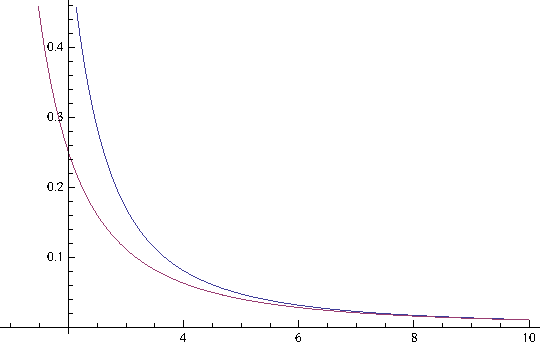
\includegraphics{series-comp-1.pdf}

Clearly $a_n$ does behave like $1/n^2$ as $n \rightarrow \infty$.  Let's prove this.
\begin{proof}
\[ n^3 + 4n + 3 < n^3 + 4n^3 + 3n^3 \]

\[ \sqrt{n^{10} + n^7} > \sqrt{n^{10}} \]

\[ \Rightarrow \frac{n^3 + 4n+3}{\sqrt{n^{10} + n^7}} < \frac{n^3 + 4n + 3}{\sqrt{n^{10}}} 
< \frac{n^3 + 4n^3 + 3n^3}{\sqrt{n^{10}}} = \frac{8n^3}{n^5} = \frac{8}{n^2} \]
Now, $\sum \frac{1}{n^2}$ converges and by Theorem~\ref{series-algebra}, $\sum \frac{8}{n^2}$ also converges.
Hence, by comparison, $\sum a_n$ converges.
\end{proof}

\item 
\[ b_n = \frac{n^3 + 4n + 3}{\sqrt{n^8 + 3n^7}} \]
As $n \rightarrow \infty$, the numerator is dominated by $n^3$ and the denominator is dominated by $\sqrt{n^8} = n^4$.  So
the sequence $b_n$ is behaving like $1/n$ suggesting divergence.

By the converse of Thorem~\ref{comparison}, we need to find a sequence smaller than $b_n$ behaving like $1/n$ indicating
divergence.

\[ n^3 < n^3 + 4n + 3 \]

\[ \sqrt{n^8 + 3n^8} > \sqrt{n^8 + 3n^7} \]

\[  \Rightarrow \frac{n^3 + 4n + 3}{\sqrt{n^8 + 3n^7}}  > \frac{n^3}{\sqrt{n^8 + 3n^7}} 
> \frac{n^3}{\sqrt{n^8 + 3n^8}} = \frac{n^3}{\sqrt{4n^8}} = \frac{1}{2n} \]
By Theorem~\ref{series-algebra}, $\sum \frac{1}{2n}$ diverges and hence $\sum b_n$ diverges by comparison.

\item
\[ c_n = \frac{n^2 - 2n}{\sqrt{n^6 + 3n^2 + 5}} \]



\end{enumerate}



%%%%%%%%%%%%%%%%%%%%%%%%%%%%%%%%%%%%%%%%%%%%%%%%%%%%%%%%%%%%%%%%%%%%%%%%

\chapter{Continuous Functions}

\[ f : D \rightarrow \mathbb{R} \;\;\; (\text{or} \; \mathbb{C}) \] 
where $D \subseteq \mathbb{R} $,  $x \in D, x \rightarrow f(x) \in \mathbb{R} $.
The set D is called the domain of the function.

\subsection{Examples of Functions}

\begin{enumerate}
	\item
	 $ f : \mathbb{R} \rightarrow \mathbb{R} \;\;\; f(x) = x^2 $.

	\item 
	$f : (0, 1)  \rightarrow \mathbb{R} \;\;\; f(x) = \frac{1}{x(x-1)} $

	\item 
	$f : \mathbb{R} \ \{0,1\} \rightarrow \mathbb{R} \;\;\; f(x) = \frac{1}{x(x-1)} $
	
	\item 
	$f : \mathbb{R} \rightarrow \mathbb{R} $
	
	\[ 
	f(x) = \left\{ \begin{array}{ll}
         x^2 & \mbox{if $x \neq 0$} \\
        1 & \mbox{if $x = 0$}
         \end{array} 
         \right. 
         \] 
         
         \item
         $f : \mathbb{R} \rightarrow \mathbb{R} $
         
         	\[ 
	f(x) = \left\{ \begin{array}{ll}
         1 & \mbox{if $x \in \mathbb{Q} $} \\
         0 & \mbox{if $x \notin \mathbb{Q} $}
         \end{array} 
         \right. 
         \] 
	
	\item
         $f : (0, \infty) \rightarrow \mathbb{R} $
         
         \[ x \in \mathbb{Q} \;\;\; x = \frac{p}{q} \;\;\; p, q \in \mathbb{Z} \;\;\; \gcd(p, q) = 1 \] 
         
         	\[ 
	f(x) = \left\{ \begin{array}{ll}
         \frac{1}{q} & \mbox{if $x \in \mathbb{Q} $} \\
         0 & \mbox{if $x \notin \mathbb{Q} $}
         \end{array} 
         \right. 
         \] 

\end{enumerate}

(3) is different from (2) since domain is different. Graph of f:

\[ \left\{ (x, f(x)) : x \in D \right\}  =  \left\{ (x, y) \in \mathbb{R}^2 :  x \in D, y = f(x) \right\} \]

We cannot really draw the graphs of (5) and (6), since rational points are dense.

\section{Behaviour of $f(x)$ for large values of $x$}

Take the function
\[ y = \frac{1}{x-2} \]
As $x$ approaches 2, taking values greater than 2, $y \rightarrow \infty$.  (Also, as $x$ approaches 2, through values less
than 2, $y \rightarrow \-infty$).  We can denote the approach of $x$ to a number $c$ through values greater than $c$ by
writing $x \rightarrow c^+$ (and through values less than $c$ by $x \rightarrow c^-$).

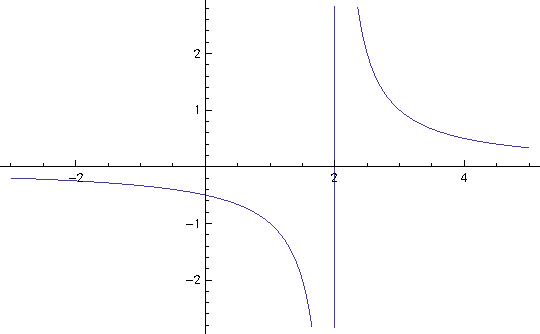
\includegraphics{func-1.pdf}

\begin{definition}
$f(x) \rightarrow \infty$ as $x \rightarrow c^+$ if, given $A$, there is $\delta$ such that 
\[ f(x) > A \;\;\; \forall x \in c < x < c + \delta \]
\end{definition}

\begin{definition}
$f(x) \rightarrow \infty$ as $x \rightarrow \infty$ if, given $A$, there exists $X$ such that
\[ f(x) > A \;\;\; \forall x > X \]
\end{definition}

\begin{definition}
$f(x) \rightarrow l$ as $x \rightarrow -\infty$ if, given $\epsilon$, there is $X$ such that 
\[ | f(x) - l | < \epsilon \;\;\; \forall x < -X \]
\end{definition}

\section{Continuous Functions}

\begin{definition}

Take a function f defined as:

\[ f : D \rightarrow \mathbb{R} \;\;\; D \subseteq \mathbb{R} \ ;\;\; a \in D \]

Then 
$\lim_{x \to a} f(x) = l \in \mathbb{R}$, if for any $\epsilon > 0$  there exists a $\delta > 0$ such that for any $x \in D$ with
$0 < |x - a| < \delta$ we have that $| f(x) - l | < \epsilon $.
We can also write this as:

\[ \lim_{x \to a} f(x) = l \iff \forall \epsilon > 0,  \exists \delta > 0: \forall x \in D, 0 < | x - a | < \delta \Rightarrow | f(x) - l | < \epsilon \]

Or, in other words, give them an $\epsilon > 0$, and they'll give a $\delta$, such that, $0 < |x - a| < \delta$, then $| f(x) - l | < \epsilon $.
\end{definition}

\subsection{Example}

Prove $\lim_{x \to 0} x^2 = 0$.

\hspace{5cm}

\begin{tikzpicture}
\begin{axis} [
    xmin=-4, xmax=5,
    ymin=-4, ymax=5,
    axis lines=center,
    axis on top=true,
    domain=-5:5,
    ]
    \addplot [mark=none,draw=red] {x*x};    
\end{axis} 
\end{tikzpicture}

\begin{proof}

Here $l = 0$.  Take $\epsilon > 0$, we want $ \left | x^2 - 0 \right | < \epsilon = \left | x^2 \right | = x^2 < \epsilon$.

\begin{eqnarray*}
x^2 < \epsilon &\Leftrightarrow&  -\sqrt{\epsilon} < x < \sqrt{\epsilon} \\
&\Leftrightarrow& |x| < \sqrt{\epsilon} 
\end{eqnarray*}

So, $\forall \epsilon > 0$, $\exists \delta$ (namely, $\delta = \sqrt{\epsilon}$), such that $|x| = |x - 0| < \delta \Leftrightarrow |x^2| = |x^2 - 0| < \epsilon$. So, $\lim_{x \to 0} x^2 = 0$.
\end{proof}

%%%%%%%%%%%%%%%%
\clearpage
\subsection{Example}

Prove $\lim_{x \to 1} x^2 = 1$.

\hspace{5cm}

\begin{tikzpicture}
\begin{axis} [
    xmin=-4, xmax=5,
    ymin=-4, ymax=5,
    axis lines=center,
    axis on top=true,
    domain=-5:5,
    ]
    \addplot [mark=none,draw=red] {x*x};    
    \addplot [mark=none,draw=blue] coordinates { (1,0) (1,4) };
    \addplot [mark=none,draw=blue] {1};    
\end{axis} 
\end{tikzpicture}

\begin{proof}
This proof is a bit more difficult than the previous one.  We have to prove:

\[ \forall \epsilon > 0,  \exists \delta > 0: 0 < | x - 1 | < \delta \Leftrightarrow | x^2 - 1 | < \epsilon \]
We want $ | x^2 - 1| $ small.  $x^2 - 1 = (x-1)(x+1)$.

\[ | x^2 - 1 | = | x - 1 | | x + 1 | \leq | x - 1 | ( 1 + |x| ) \]

since, using the triangle inequality, we can write:

\[ | x + 1 | \leq | x | + 1 \]

Now observe that if $ | x - 1 |  < 1 \Rightarrow | x | < 2$, since 

\[ | x | = | x - 1 + 1 | \]
This follows from the triangle inequality:
\[ | x - 1 + 1 |  \leq | x - 1 | + |1| = |x - 1| + 1 < 2 \]




\end{proof}

%%%%%%%%%%%%%%%%
\clearpage
\subsection{Example}

Prove $\lim_{x \to 1} \frac{3x(x-1)}{(x-1)} = 3$.
Or in other words, 
prove: Given $\epsilon > 0$, I can give a $\delta > 0$ as long as $ 0 < | x - 1 | < \delta $, then 
$ \left | \frac{3x(x-1)}{(x-1)} - 3 \right | < \epsilon $.

\begin{proof}
We start where we want to get to:

\[ \left | \frac{3x(x-1)}{(x-1)} - 3 \right | < \epsilon \]

As long as $x \ne 1$ (which is OK since we only consider the case of x approaching 1), we can cancel out $(x - 1)$:

\begin{eqnarray*}
&\Leftrightarrow&  \left | 3x - 3 \right |  < \epsilon \\
&\Leftrightarrow& \left | 3 (x - 1) \right |  < \epsilon \\
&\Leftrightarrow& \left | 3 \right | \left | x - 1 \right | < \epsilon \\
&\Leftrightarrow& 3 \left | x - 1 \right | < \epsilon \\
&\Leftrightarrow& \left | x - 1 \right | < \frac{\epsilon}{3} 
\end{eqnarray*}

So, we can use $\frac{\epsilon}{3}$ as our $\delta$.  For example, if you give me an $\epsilon = 1$, then what this means is that

\[ \left | \frac{3x(x-1)}{(x-1)} - 3 \right | < 1 \Leftrightarrow \left | x-1\right | < \frac{1}{3} \]

i.e. as long as $x$ is within $\frac{1}{3}$ of 1, then distance between the function and 3 will be less than 1.

\end{proof}

\begin{tikzpicture}
\begin{axis} [
    xmin=-4, xmax=5,
    ymin=-4, ymax=5,
    axis lines=center,
    axis on top=true,
    domain=-5:5,
    ]

    \addplot [mark=none,draw=red,ultra thick] {3*x};    
    \addplot [mark=none,draw=blue] {3};   
    \addplot [mark=none,draw=blue]  coordinates { (1,0) (1,3) };
    
    \addplot [mark=none,draw=green] coordinates { (2/3,0) (2/3,2) };
    \addplot [mark=none,draw=green] coordinates { (4/3,0) (4/3,4) };
    
    \addplot [mark=none,draw=brown] coordinates { (0,2) (3,2) };
    \addplot [mark=none,draw=brown] coordinates { (0,4) (3,4) };
\end{axis} 
\end{tikzpicture}

%%%%%%%%%%%%%%%%%%%%%%%%%%%%%%%%%%%%%%%%%%%%%%%%%%%%%%%%%%%%%%%%%%%%%%%%
\clearpage
\chapter{Complex Numbers}

\end{document}